\providecommand{\main}{..}
\documentclass[\main/thesis.tex]{subfiles}

\begin{document}


\chapter{Benchmark Results}

We compare the KL methods on benchmark continuous and discrete-action environments, using non-linear function approximation. Here, we wish to understand (1) if our observations from the microworld experiments apply to more complicated environments and (2) if any new differences as a result of function approximation or increased environment complexity. 

\section{Implementation Details}
\subsection{Hyperparameters}
Hyperparameter sweeps are performed separately for each domain. We sweep over the learning rates $\{10^{-5}, 10^{-4}, 10^{-3}\}$; for Pendulum, we additionally sweep over actor learning rate $10^{-2}$. In the continuous-action setting, we sweep both the actor and the critic learning rate, while in the discrete-action setting we have a shared learning rate because of a shared architecture. We sweep temperatures in $\{0.01, 0.1, 1\}$ for the soft action-value methods and set the temperature in $\boltzmannQ$ and the temperature in the soft action-value function to be the same value. For example, if $\tau = 0.01$, then we learn a soft action-value function with $\tau = 0.01$ and use a KL target distribution proportional to $\exp(Q(s, a) \tau^{-1})$. RMSprop \citep{tieleman2012lecture} is used as the optimizer to be consistent with our focus in the microworld domains. 

We perform 30 runs for all hyperparameter settings and plot the mean return averaged over the past 20 episodes; shaded areas represent standard errors. 


\subsection{Updating}
We perform bootstrapping as per the recommendations in \citet{pardo2017time}. If a transition $(s, a, r, sp)$ results in the true termination of the episode, the bootstrap target for value function updates is $r$ instead of the usual $r - \tau \log \pi(a \mid s) + \gamma V(sp)$. If the transition results in a timeout, $r - \tau \log \pi(a \mid s) + \gamma V(sp)$ is used. Otherwise, $r - \tau \log \pi(a \mid s) + \gamma V(sp)$ is used as the bootstrap target. 

On the continuous-action domains we use Clenshaw-Curtis \citep{clenshaw1960method} numerical integration scheme to estimate the FKL and the RKL. To generate the points for Clenshaw-Curtis, we use the Python package, quadpy.\footnote{\url{https://github.com/nschloe/quadpy}}. For computational efficiency, we use 64 points for 1D environments, and $l=6$ for multi-dimensional environments using the nested univariate quadrature formula for Clenshaw-Curtis \citep{gerstner1998numerical}. In learning value functions we learn both $Q(s, a)$ and $V(s)$, using the same target as done in SAC \citep{haarnoja2018soft}. In particular, the target for $V(s)$ is $Q(s, a) - \log(\pi(a \mid s))$. On preliminary experiments, we found that the target of $Q(s, a) - \log(\pi(a \mid s))$ performed better than the target of $r(s) - \tau \log \pi(a \mid s) + \gamma V(s')$ for all methods.

On the discrete-action domains, the value function update target is $r(s) - \tau \log \pi(a \mid s) + \gamma V(s')$ instead of the update that SAC uses, $Q(s, a) - \log \pi(a \mid s)$. Preliminary experiments indicated that the former update was superior for all methods. Both $Q$ and $V$ are learned. 

For reference, we also include the gradient updates of the various KL divergences. 
\begin{align}
    &\textbf{RKL}: \nabla_\theta \KL(\pi_\theta(\cdot \mid s) \parallel \boltzmannQ_\tau(s, \cdot)) \nonumber\\
    &\quad= -\nabla_\theta \entropy(\pi_\theta(\cdot \mid s)) - \int_\actionspace\nabla_\theta \pi_\theta(a \mid s) \log \boltzmannQ_\tau(a \mid s)\, da \label{eq:rkl-gradient}\\
    &\textbf{FKL}: \nabla_\theta \KL(\boltzmannQ_\tau(s, \cdot) \parallel \pi_\theta(\cdot \mid s) )\nonumber\\
    &\quad= - \int_\actionspace  \boltzmannQ_\tau(a \mid s) \nabla_\theta \log \pi_\theta(a \mid s) \, da \label{eq:fkl-gradient} \\
    &\textbf{Hard RKL}: - \int_\actionspace\nabla_\theta \pi_\theta(a \mid s) Q(s, a)\, da \label{eq:hrkl-gradient}\\
    &\textbf{Hard FKL}: -\nabla_\theta \log \pi_\theta \left(\argmax_b Q(s, b) \mid s\right) \label{eq:hfkl-gradient}.
\end{align}

\begin{algorithm}
\caption{Agent for Benchmark Experiments}
\label{alg:kl-agent}
\begin{algorithmic}
    \State Given: policy $\pi_\theta$ (parameters $\theta$); action-value estimate $Q_v$ (parameters $v$); state-value estimate $V_w$ (parameters $w$); experience replay buffer; choice of KL divergence; temperature $\tau \geq 0$; learning rates for $\theta$, $v$, $w$; optimizer (e.g., RMSprop).
    \For{$t = 0, \ldots,$}
        \State Draw action $a_t \sim \pi_\theta(\cdot \mid s_t)$
        \State Observe and store transition $(s_t, a_t, s_{t + 1}, r, \text{DoneFlag})$. Replace the oldest transition if the buffer size limit is reached. 
        \If{samples in buffer $\geq$ 32}
            \State Draw random mini-batch of size 32 from buffer. 
            \For{each transition $(s, a, r, sp, \text{DoneFlag})$ in the mini-batch}
                \State Calculate KL gradients according to \Cref{eq:rkl-gradient,eq:fkl-gradient,eq:hrkl-gradient,eq:hfkl-gradient}, based on choice of $\tau$ and KL divergence.
            \EndFor
            \State Update $w, v$ with DiscreteUpdateValueFunctions if action space is discrete; otherwise call ContinuousUpdateValueFunctions.
            \State Update $\theta$ with the learning rate and optimizer.
        \EndIf
    \EndFor
\end{algorithmic}
\end{algorithm}

\begin{algorithm}
\caption{DiscreteUpdateValueFunctions}
\label{alg:discrete-value-update}
\begin{algorithmic}
    \State Given: policy $\pi_\theta$ (parameters $\theta$); action-value estimate $Q_v$ (parameters $v$); state-value estimate $V_w$ (parameters $w$); temperature $\tau \geq 0$;  optimizers (e.g., RMSprop) for $v$ and $w$; batch of data $\mathcal{D}$, with each transition written in the form $(s, a, r, sp, \text{DoneFlag})$
    \State To update the state-value function, pass the following as the gradient to the optimizer for $w$. 
    \begin{align*}
        -\Ex_{\mathcal{D}}[(r - \tau \log \pi(a \mid s) + \gamma\cdot (1 - \text{DoneFlag})\cdot V_w(sp) - V(s)) \nabla_w V(s)]
    \end{align*}
    \State To update the action-value function, pass the following as the gradient to the optimizer for $v$. 
    \begin{align*}
        -\Ex_{\mathcal{D}}[(r + \gamma \cdot (1 - \text{DoneFlag})\cdot V_w(sp) - Q_v(s, a)) \nabla_v Q_v(s, a)]
    \end{align*}
\end{algorithmic}
\end{algorithm}

\begin{algorithm}
\caption{ContinuousUpdateValueFunctions}
\label{alg:continuous-value-update}
\begin{algorithmic}
    \State Given: policy $\pi_\theta$ (parameters $\theta$); action-value estimate $Q_v$ (parameters $v$); state-value estimate $V_w$ (parameters $w$); temperature $\tau \geq 0$; optimizers (e.g., RMSprop) for $v$ and $w$; batch of data $\mathcal{D}$, with each transition written in the form $(s, a, r, sp, \text{DoneFlag})$
    \State For each state $s$ in the batch $\mathcal{D}$, draw a new action $\tilde{a} \sim \pi_\theta(\cdot \mid s)$.
    \State To update the state-value function, pass the following as the gradient to the optimizer for $w$. 
    \begin{align*}
        \Ex_{\mathcal{D}}[(V_w(s) - Q_v(s, \tilde{a}) + \tau \log \pi_\theta (\tilde{a} \mid s)) \nabla V_w(s)]
    \end{align*}
    \State To update the action-value function, pass the following as the gradient to the optimizer for $v$. 
    \begin{align*}
        -\Ex_{\mathcal{D}}[(r + \gamma \cdot (1 - \text{DoneFlag})\cdot V_w(sp) - Q_v(s, a)) \nabla_v Q_v(s, a)]
    \end{align*}
\end{algorithmic}
\end{algorithm}

In all our plots, we refer to the number of ``frames'' on the $x$-axis. We use ``frames'' synonomously with ``timestep''. 

\subsection{Architecture}
On our continuous-action domains, all policy and value function networks are implemented as two-layer neural networks of size 128, with ReLU activations. We use experience replay of buffer size $10^6$ with batch size of 32. On our discrete-action domains, we employ the following architectures.

\textbf{OpenAI Gym}: The architecture is a two-layer neural network, with the policy and value functions as separate heads off of the main two-layer body. ReLU activations are used between layers. We report results for three hidden layer sizes: small (32), medium (128), and large (512).

\textbf{MinAtar}: The architecture is a convolutional network into one fully-connected layer for each of the policy, action value function, and state value function. The convolutional layer has 16 3x3 convolutions with stride 1, the same as in \citet{young2019minatar}; we vary the size of the fully-connected layer in $\{32, 128\}$. ReLU activations are used between layers. 

On the discrete-action domains, experience replay is used with a buffer size of $10^5$ and a batch size of 32. 

\section{Continuous-Action Results}
We compare agents on Pendulum \citep{brockman2016openai}, Reacher, and Swimmer \citep{todorov2012mujoco}, with results shown in Figure \ref{fig_cont}. We exclude Hard FKL in our comparison since it requires access to $\max_a Q(s,a)$, which is difficult to obtain with continuous actions. 


\begin{figure}[t]
  \centering
  \begin{subfigure}[b]{0.5\linewidth}
    \centering
    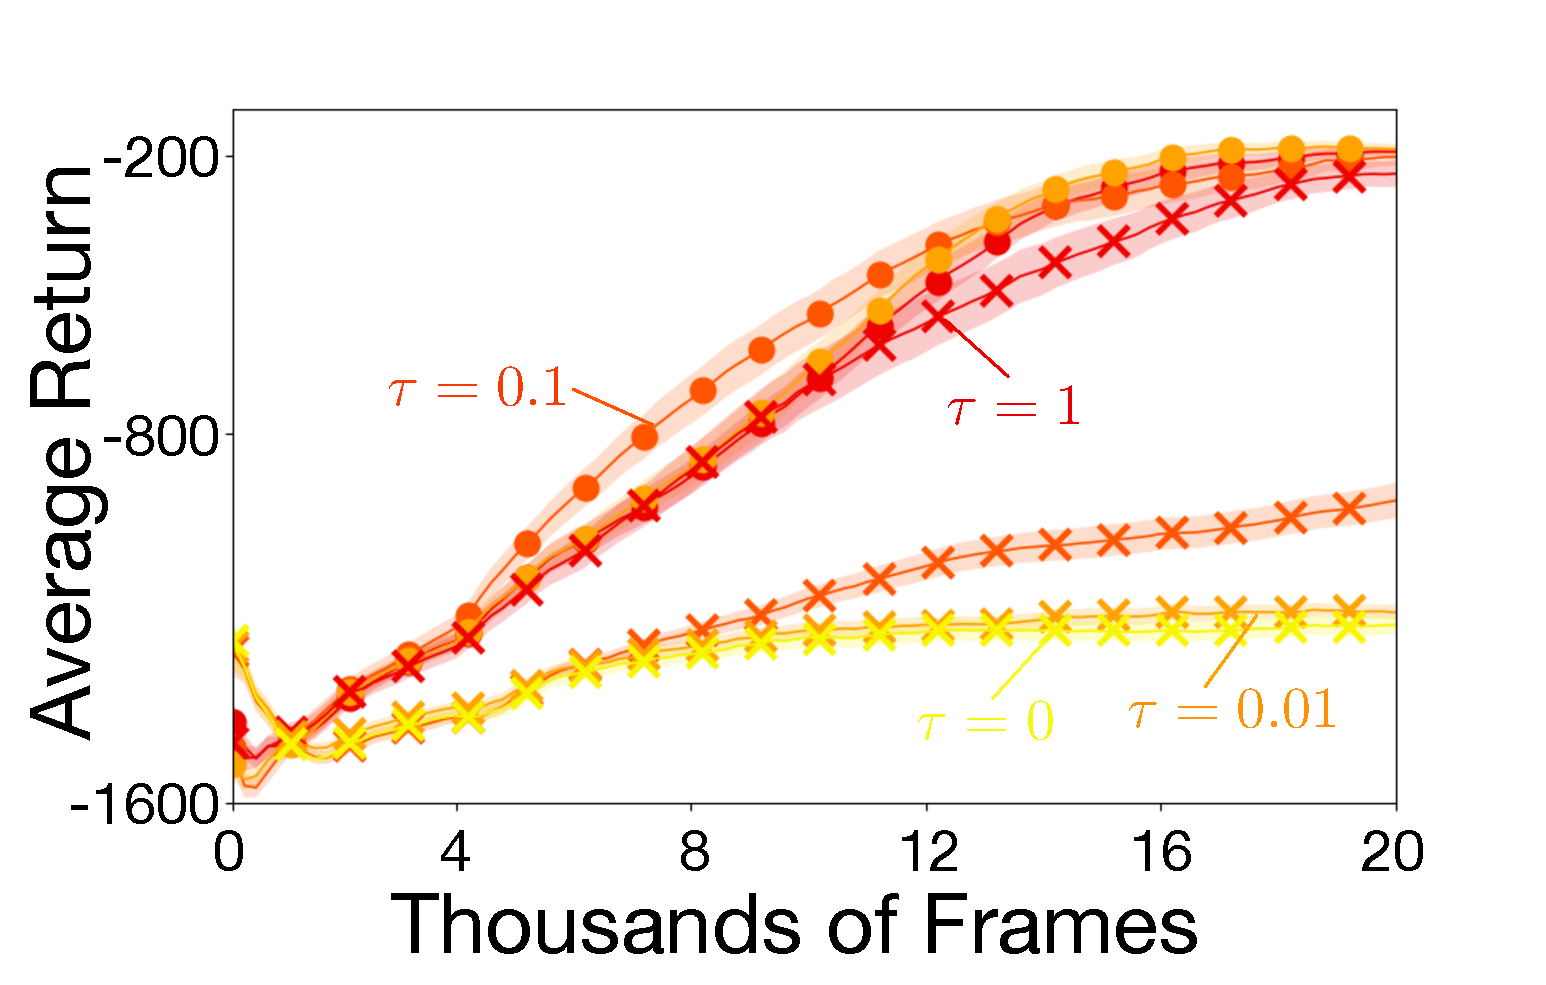
\includegraphics[width=\columnwidth]{figs/deep/continuous/PD_entropy_comparison.pdf} 
    \caption{Pendulum}\label{fig:pendulum}
  \end{subfigure}%
  \begin{subfigure}[b]{0.5\linewidth}
    \centering
    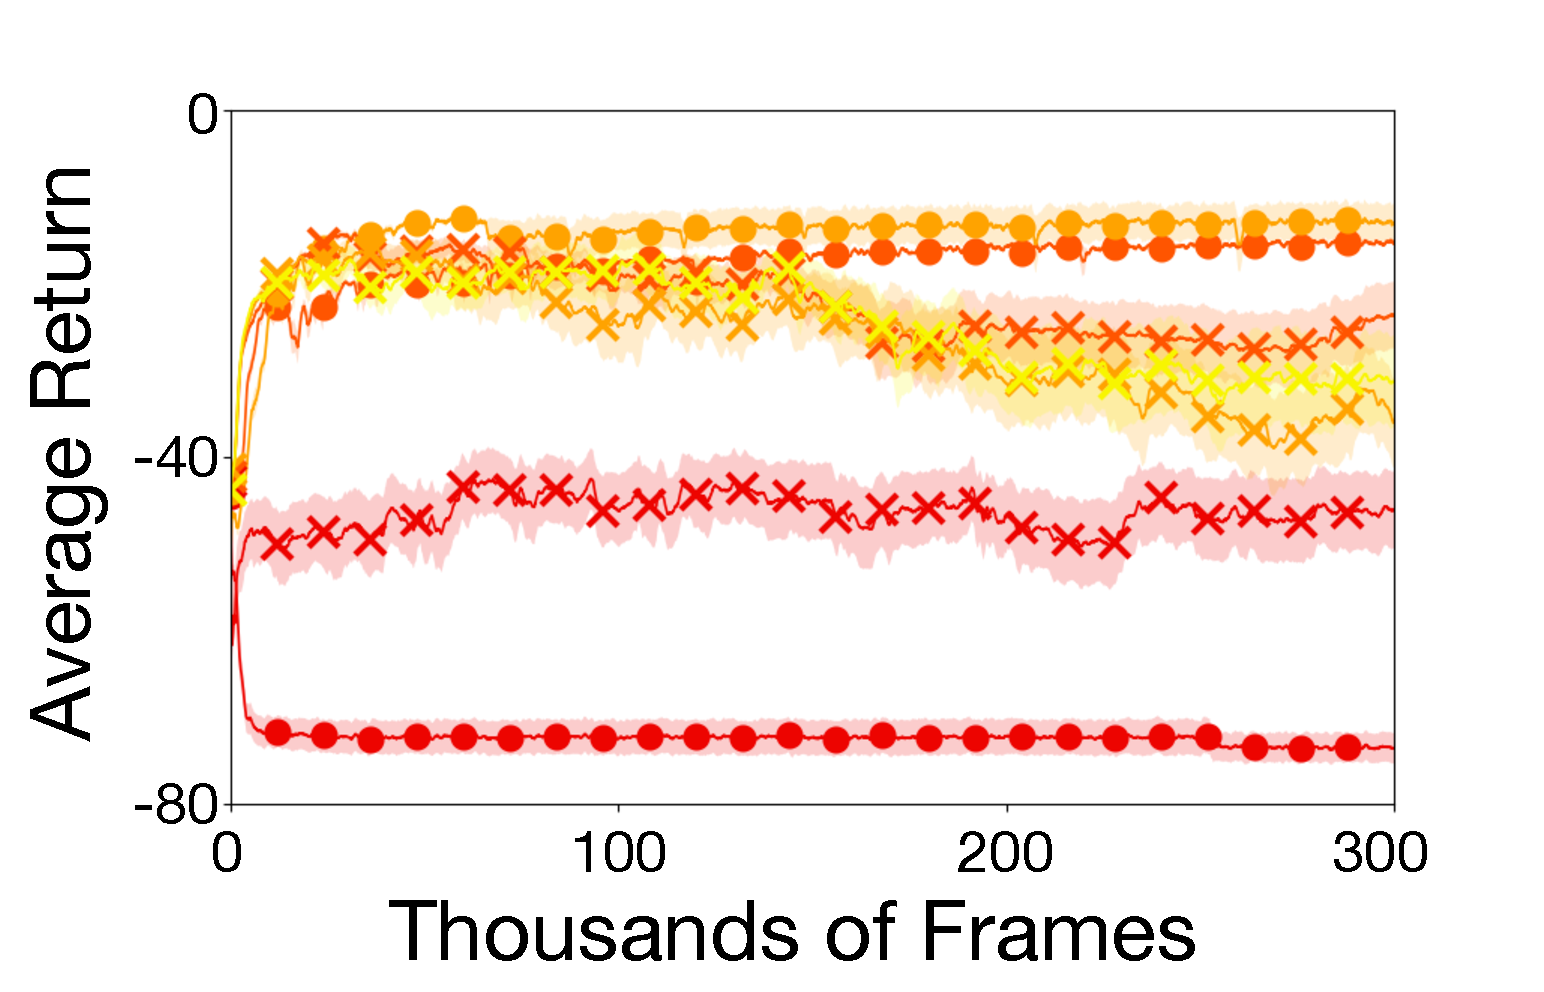
\includegraphics[width=\columnwidth]{figs/deep/continuous/Reacher_entropy_comparison.pdf} 
    \caption{Reacher}\label{fig:reacher}
  \end{subfigure}
  
  \begin{subfigure}[b]{0.5\linewidth}
    \centering
    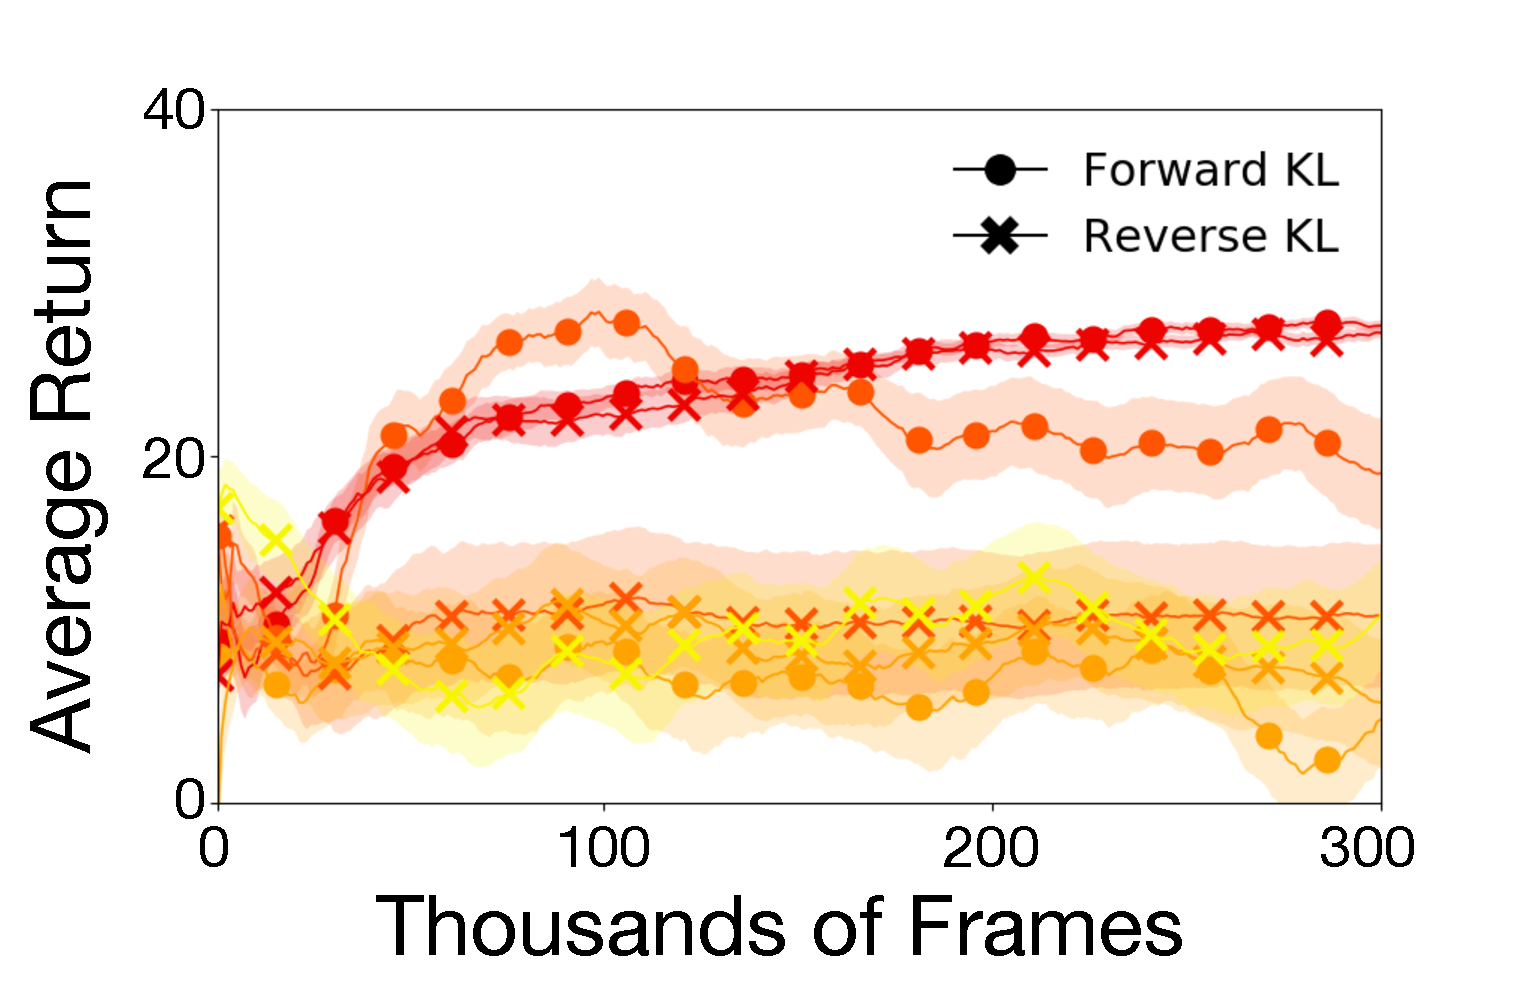
\includegraphics[width=\columnwidth]{figs/deep/continuous/Swimmer_entropy_comparison.pdf} 
    \caption{Swimmer}\label{fig:swimmer}
  \end{subfigure}
  \caption{Continuous-action environments. Shown are the best hyperparameters for each algorithm, which are selected by largest area under the last half of the learning curve. The colours go from hot (red, temperature = 1) to cool (yellow, temperature = 0). }\label{fig_cont}
\end{figure}

For certain temperatures, FKL either learns faster than or achieves superior final return to RKL. This difference is especially striking on Pendulum \Cref{fig:pendulum}, where FKL learns vastly faster than RKL for $\tau = 0.1, 0.01$. It's interesting to note that RKL with $\tau = 1$ has a similarly-shaped learning curve to FKL with $\tau = 0.01, 0.1, 1$. In a sense, the higher temperature of RKL with $\tau = 1$ might be compensating for committal behaviour of RKL that we observed in the microworld experiments. It does seem possible to be too non-committal. On Reacher in \Cref{fig:reacher}, FKL with $\tau = 1$ completely fails to learn, while all other settings learn appreciably. Nevertheless, these observations suggest a connection between the impacts of FKL and of entropy regularization, as we discuss further below in the discrete-action setting. 

It is difficult to comment on the importance of the policy parameterization for these experiments relative to our microworld experiments. Any influence from the Gaussian policy parameterization is conflated with function approximation. Moreover, as we will see below, no stark pattern seems to divide continuous and discrete action settings, as one did in our microworld experiments. 

\section{Discrete-Action Results}
We report results for environments from the OpenAI gym \citep{brockman2016openai} and MinAtar \citep{young2019minatar}. 



\begin{figure}[t]
  \centering
  \begin{subfigure}[b]{1\linewidth}
    \centering
    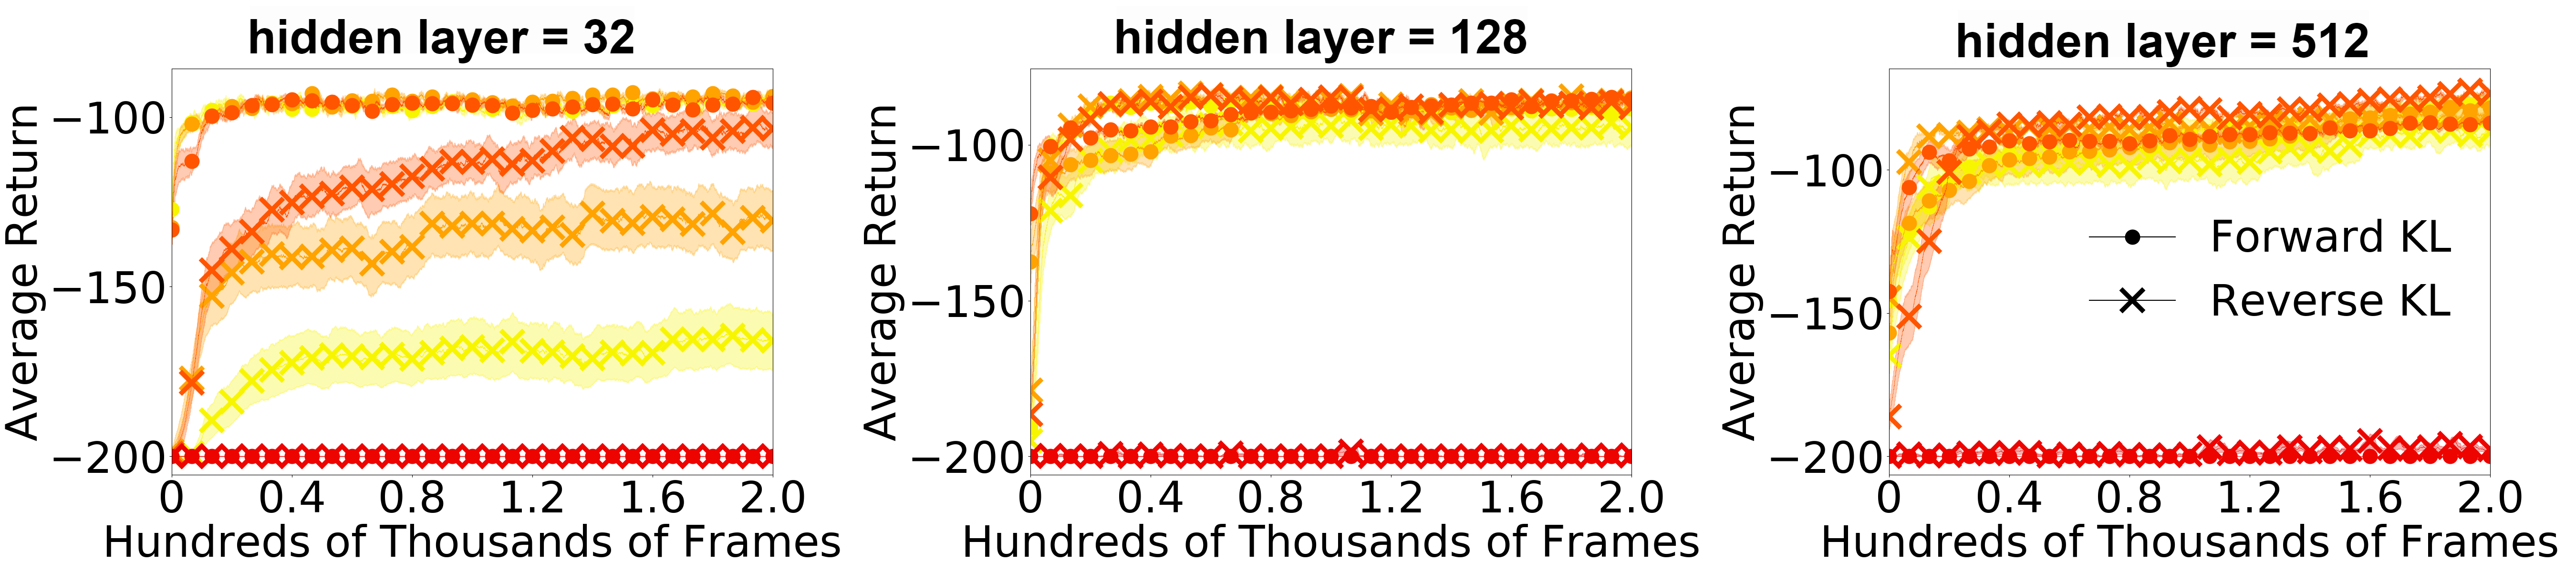
\includegraphics[width=\columnwidth]{figs/deep/discrete/acrobot_combined.png} 
    \caption{Acrobot}\label{fig:acrobot}
  \end{subfigure}%
  
  \begin{subfigure}[b]{1\linewidth}
    \centering
    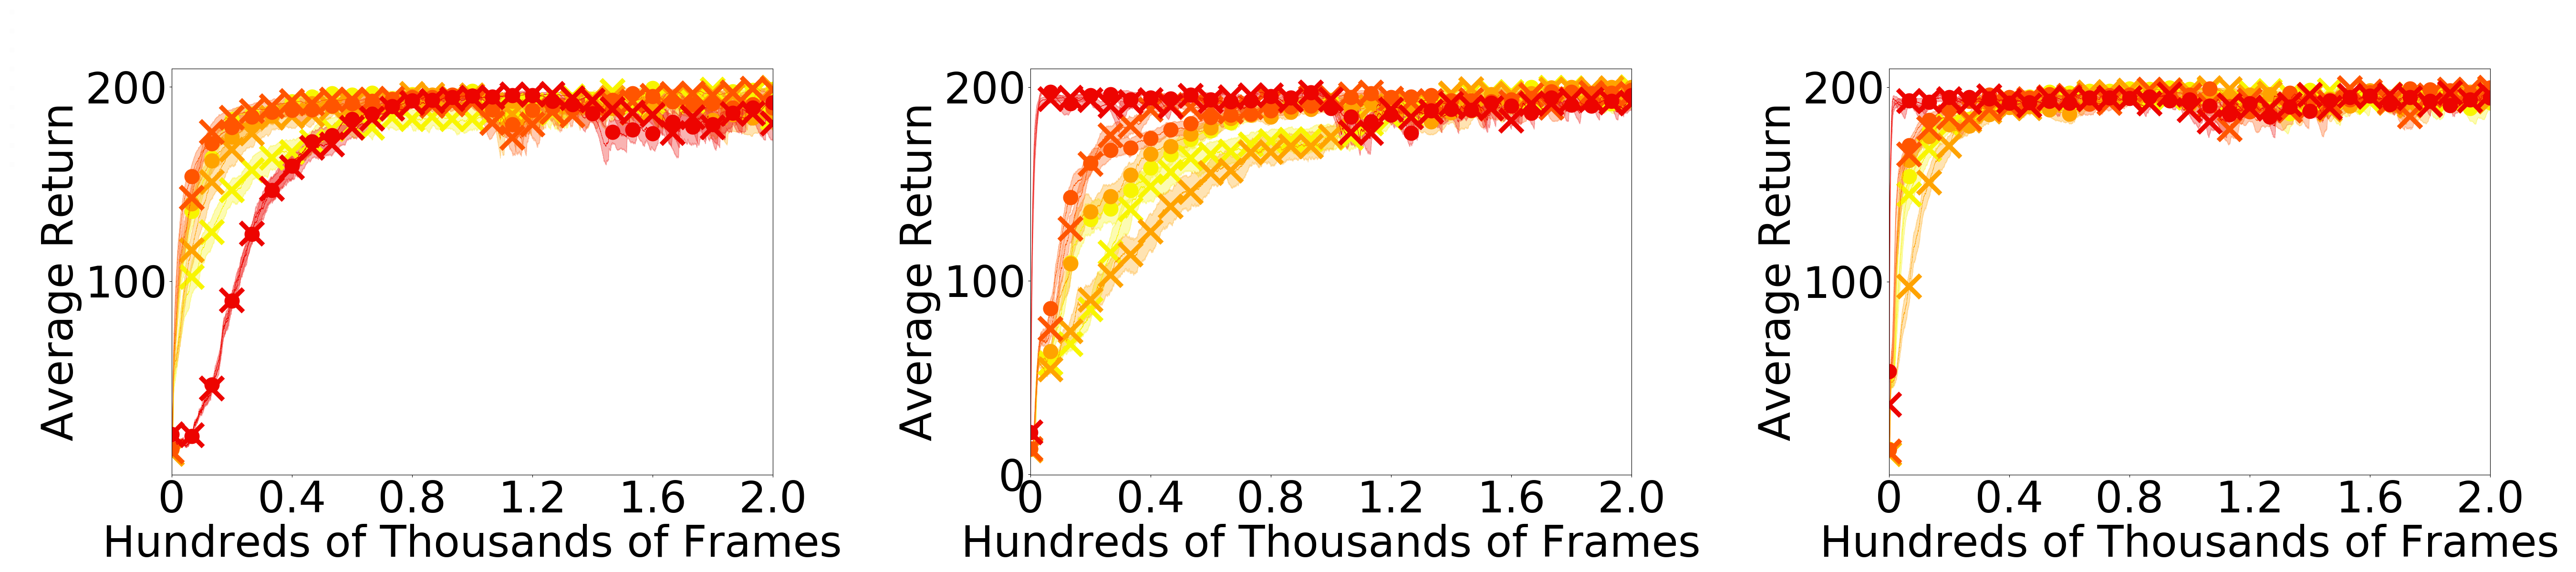
\includegraphics[width=\columnwidth]{figs/deep/discrete/cartpole_combined.png}
    \caption{CartPole}\label{fig:cartpole}
  \end{subfigure}
  
  \begin{subfigure}[b]{1\linewidth}
    \centering
    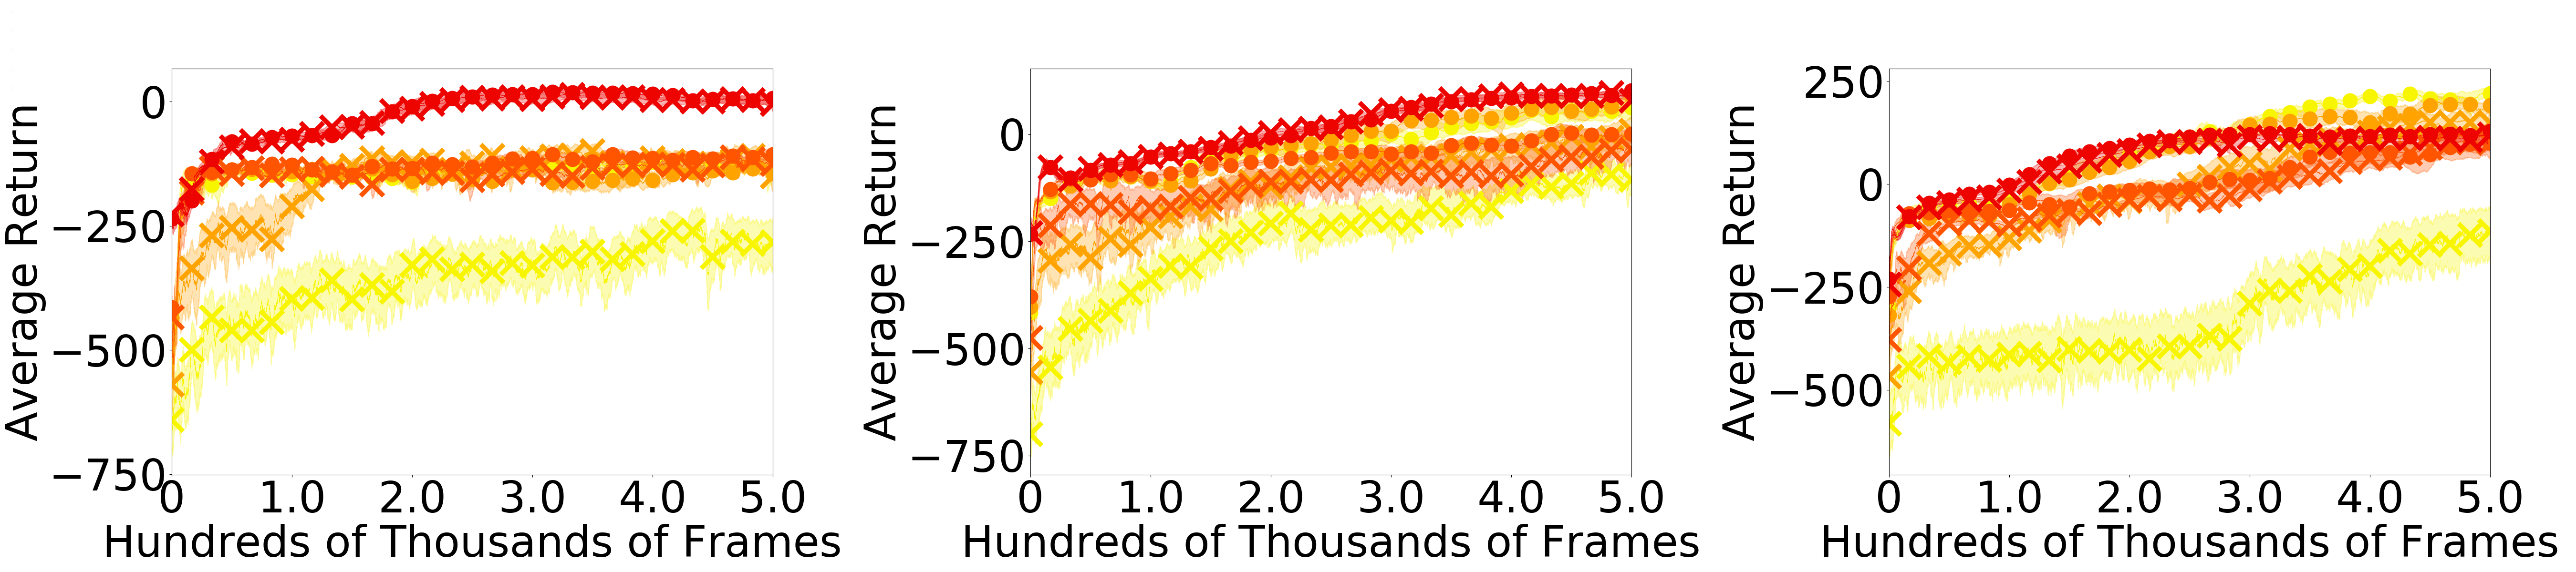
\includegraphics[width=\columnwidth]{figs/deep/discrete/lunar_combined.png}
    \caption{Lunar Lander.}
    \label{fig:lunar-lander}
  \end{subfigure}
  \caption{OpenAI Gym discrete-action environments. Plot settings are identical to Figure \ref{fig_cont}.}\label{fig:open-ai}
\end{figure}

% In Acrobot, FKL dominates RKL for all temperatures except $\tau = 1$, which did not learn at all.  This last trend could be because RKL ``commits'' more to actions with high density (i.e., have lower standard deviation, all other things being equal), which we observed in the microworld experiments as well. In CartPole, FKL at $\tau = 0.01, 0.1$ seems to learn a little bit faster than CartPole for hidden layer size $= 128, 256$. In Lunar Lander, FKL with non-zero temperature consistently matches or exceeds the corresponding learning curve for RKL. Indeed, when $\tau = 0$, a large gap separates FKL and RKL. A possible reason  

The results on the OpenAI Gym environments suggest that for small hidden layer sizes, FKL may be at least as good as RKL, and sometimes better. As the hidden layer size increases, however, this dominance is negated. For a hidden layer size of 128, RKL seems to learn a little bit faster than FKL for $\tau \neq 1$, and RKL has a slightly higher final performance for a hidden layer size of 512, although the difference does not appear to be significant. It is possible that these observations are related to how the optimization landscape of a neural network changes with larger hidden layer sizes. The influence of the choice of policy gradient objective on the optimal function approximation architecture deserves further consideration. 

The superiority of FKL in Lunar Lander for $\tau = 0, 0.01$ and sometimes $\tau = 0.1$ is interesting. For these temperatures, FKL with non-zero temperature consistently matches or exceeds the corresponding learning curve for RKL. Indeed, when $\tau = 0$, a large gap separates FKL and RKL. A possible reason for this dominance is the difficulty of exploration in Lunar Lander: one must learn to manoeuvre the spacecraft, discover the correct landing area, learn how to land correctly, and learn to turn off the fuel. That FKL might ``commit'' less (i.e., have higher standard deviation than RKL, all other things equal) suggests that more actions are tried to facilitate discovery of good actions. We further discuss exploration below in our MinAtar experiments. 

\begin{figure}[!htb]
  \centering
  \begin{subfigure}[b]{1\linewidth}
    \centering
    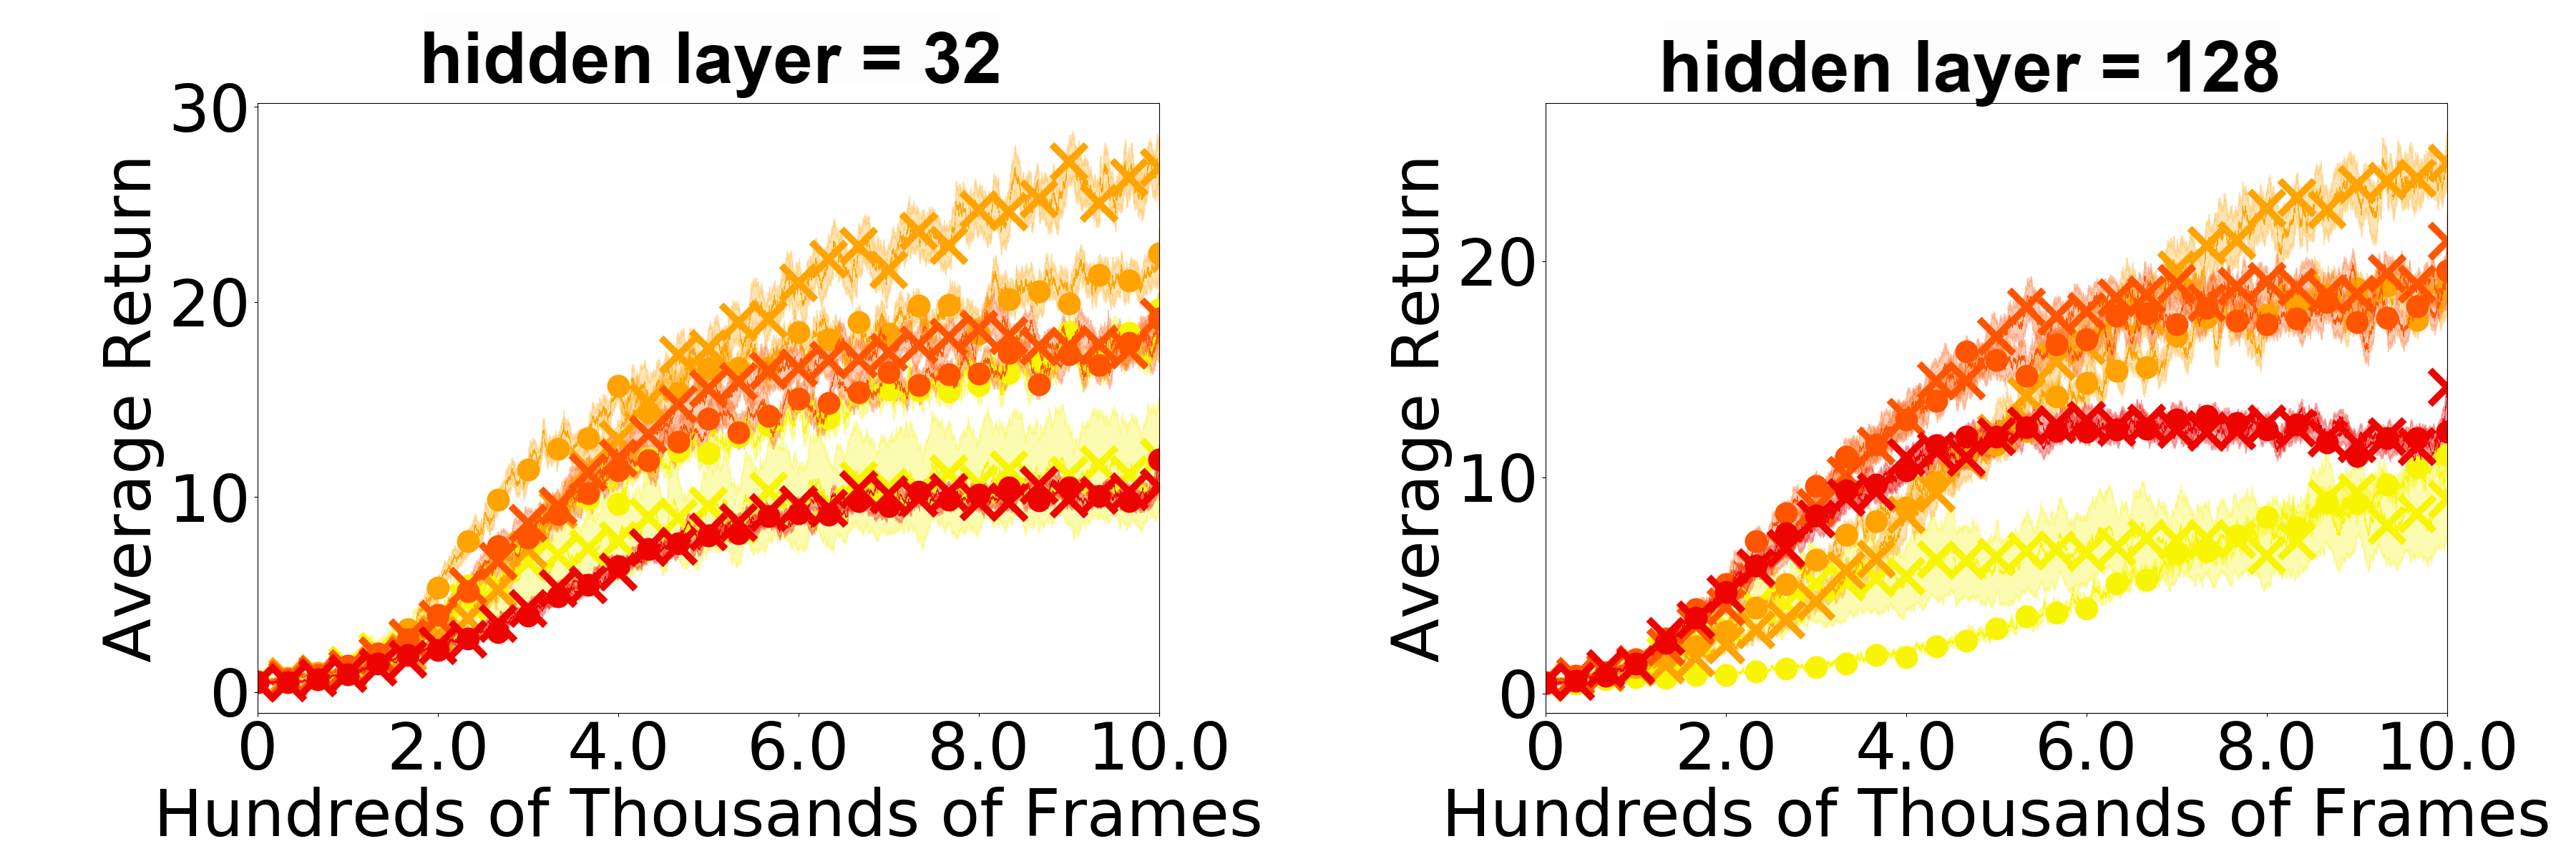
\includegraphics[width=\columnwidth]{figs/deep/discrete/asterix_combined.png} 
    \caption{Asterix
    }\label{fig:asterix}
  \end{subfigure}%
  
  \begin{subfigure}[b]{1\linewidth}
    \centering
    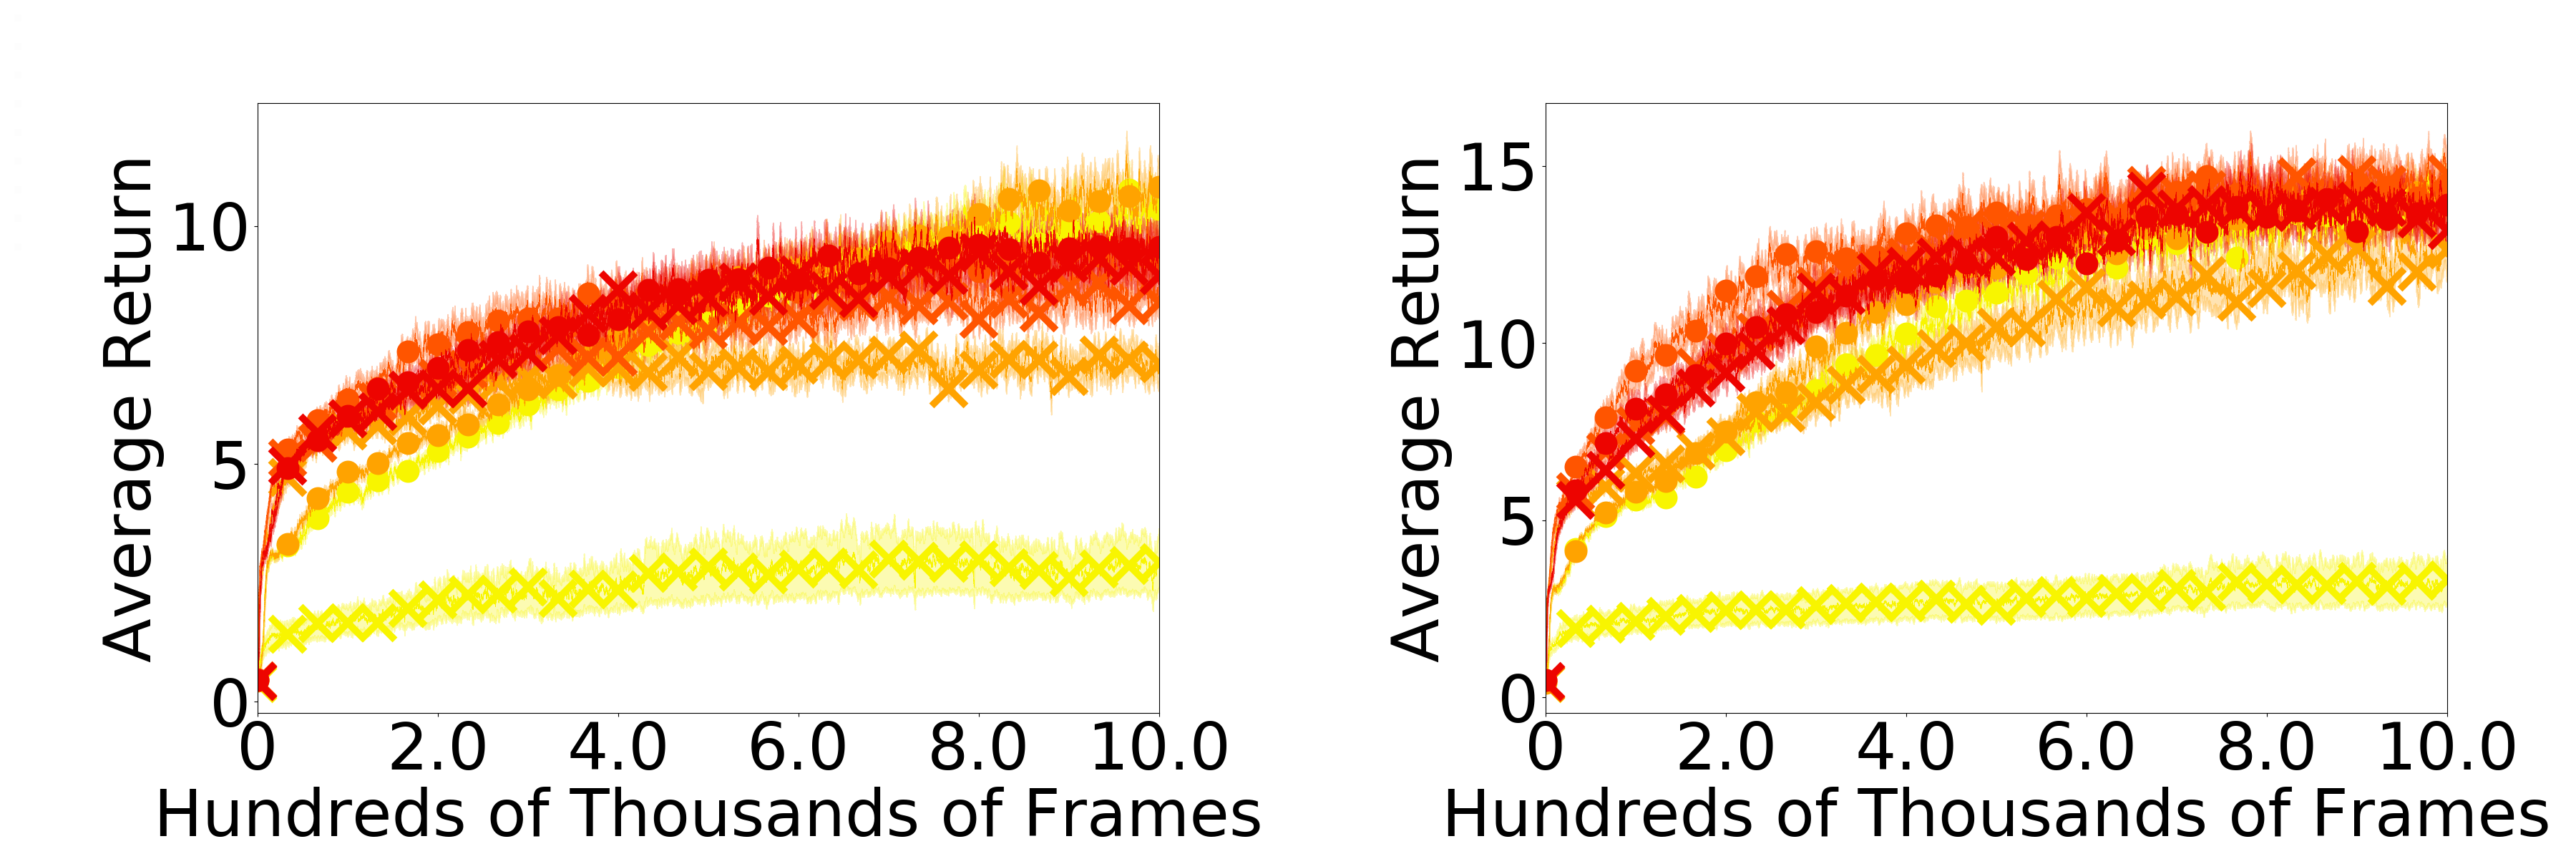
\includegraphics[width=\columnwidth]{figs/deep/discrete/breakout_combined.png} 
    \caption{Breakout
    }\label{fig:breakout}
  \end{subfigure}%
  
  \begin{subfigure}[b]{1\linewidth}
    \centering
    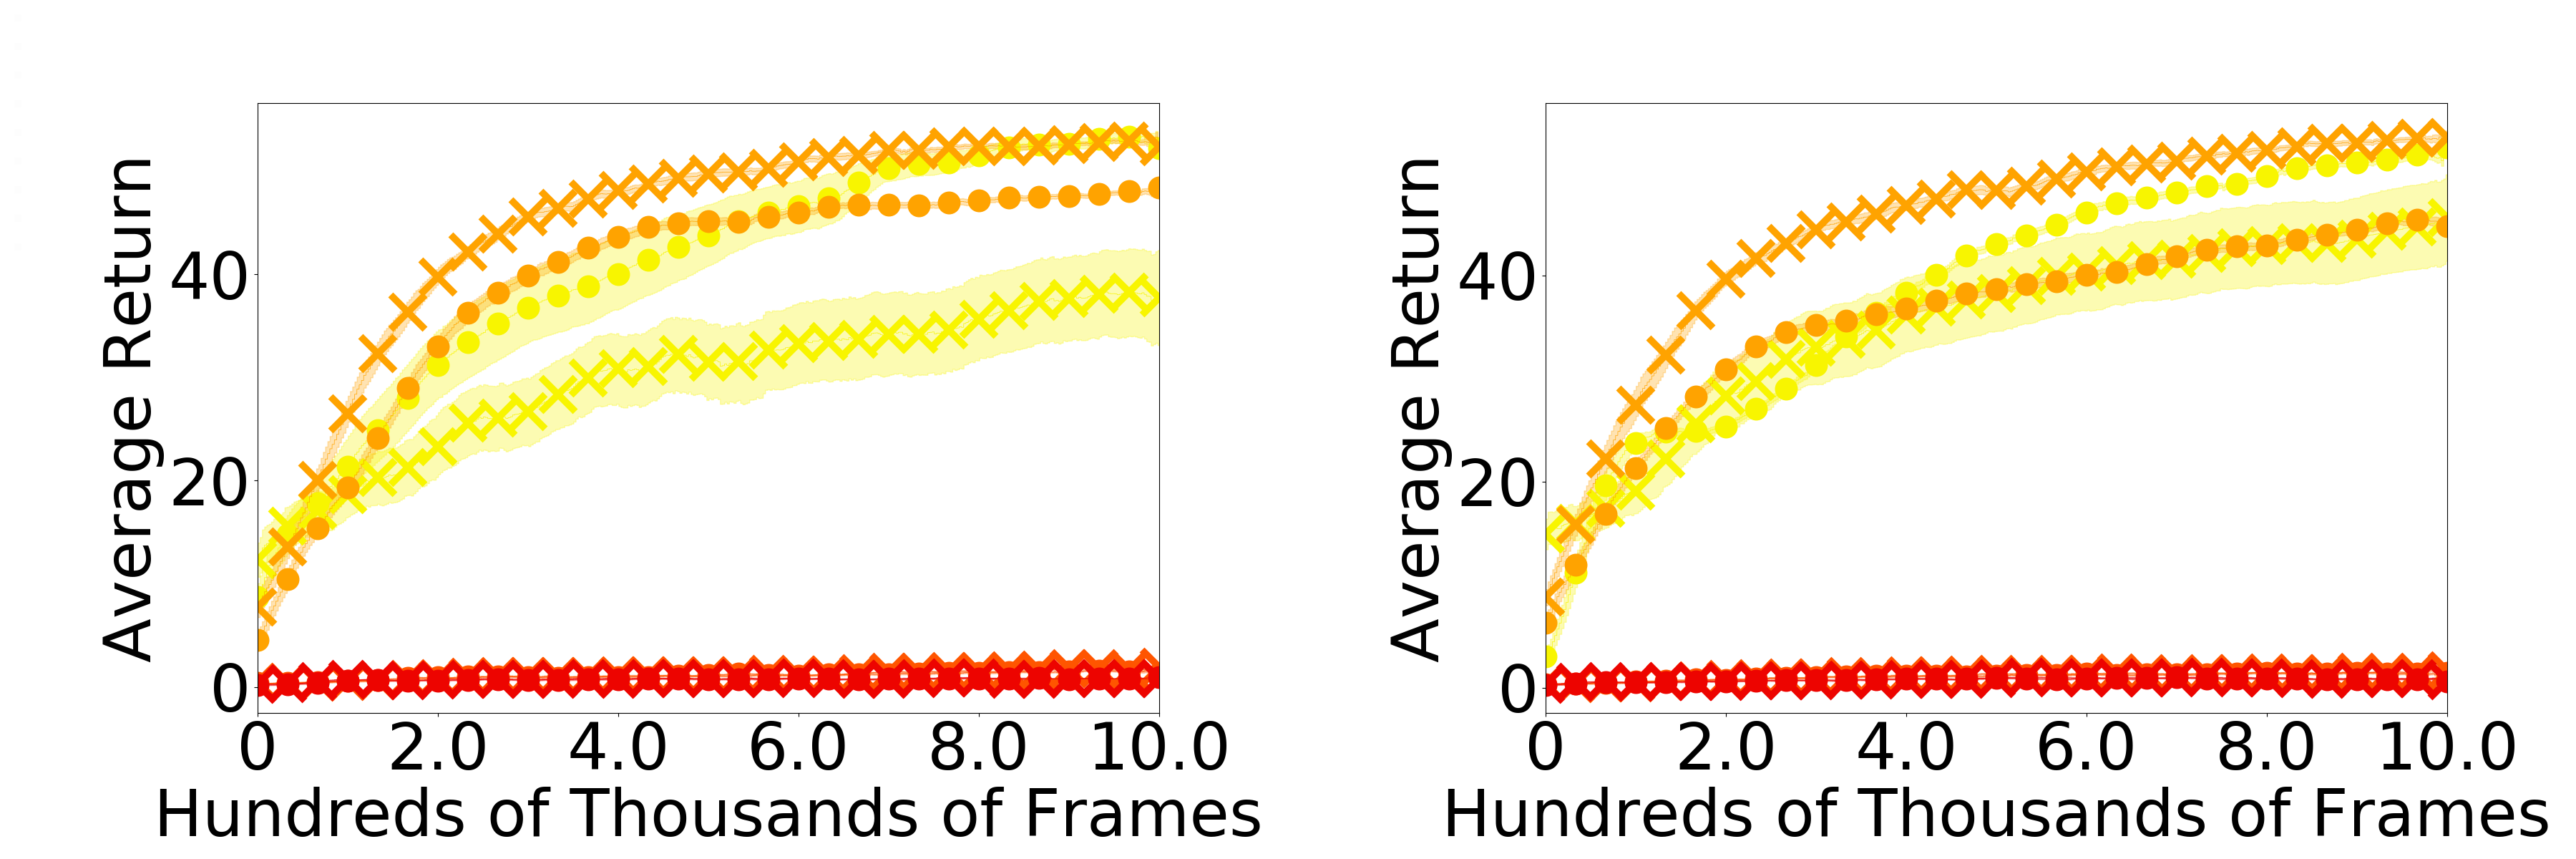
\includegraphics[width=\columnwidth]{figs/deep/discrete/freeway_combined.png} 
    \caption{Freeway
    }\label{fig:freeway}
  \end{subfigure}%
  \caption{MinAtar discrete-action environments. Plot settings are identical to those in Figure \ref{fig_cont}. }\label{fig:minatar}
\end{figure}
\begin{figure}[!htb]
  \begin{subfigure}[b]{1\linewidth}
    \centering
    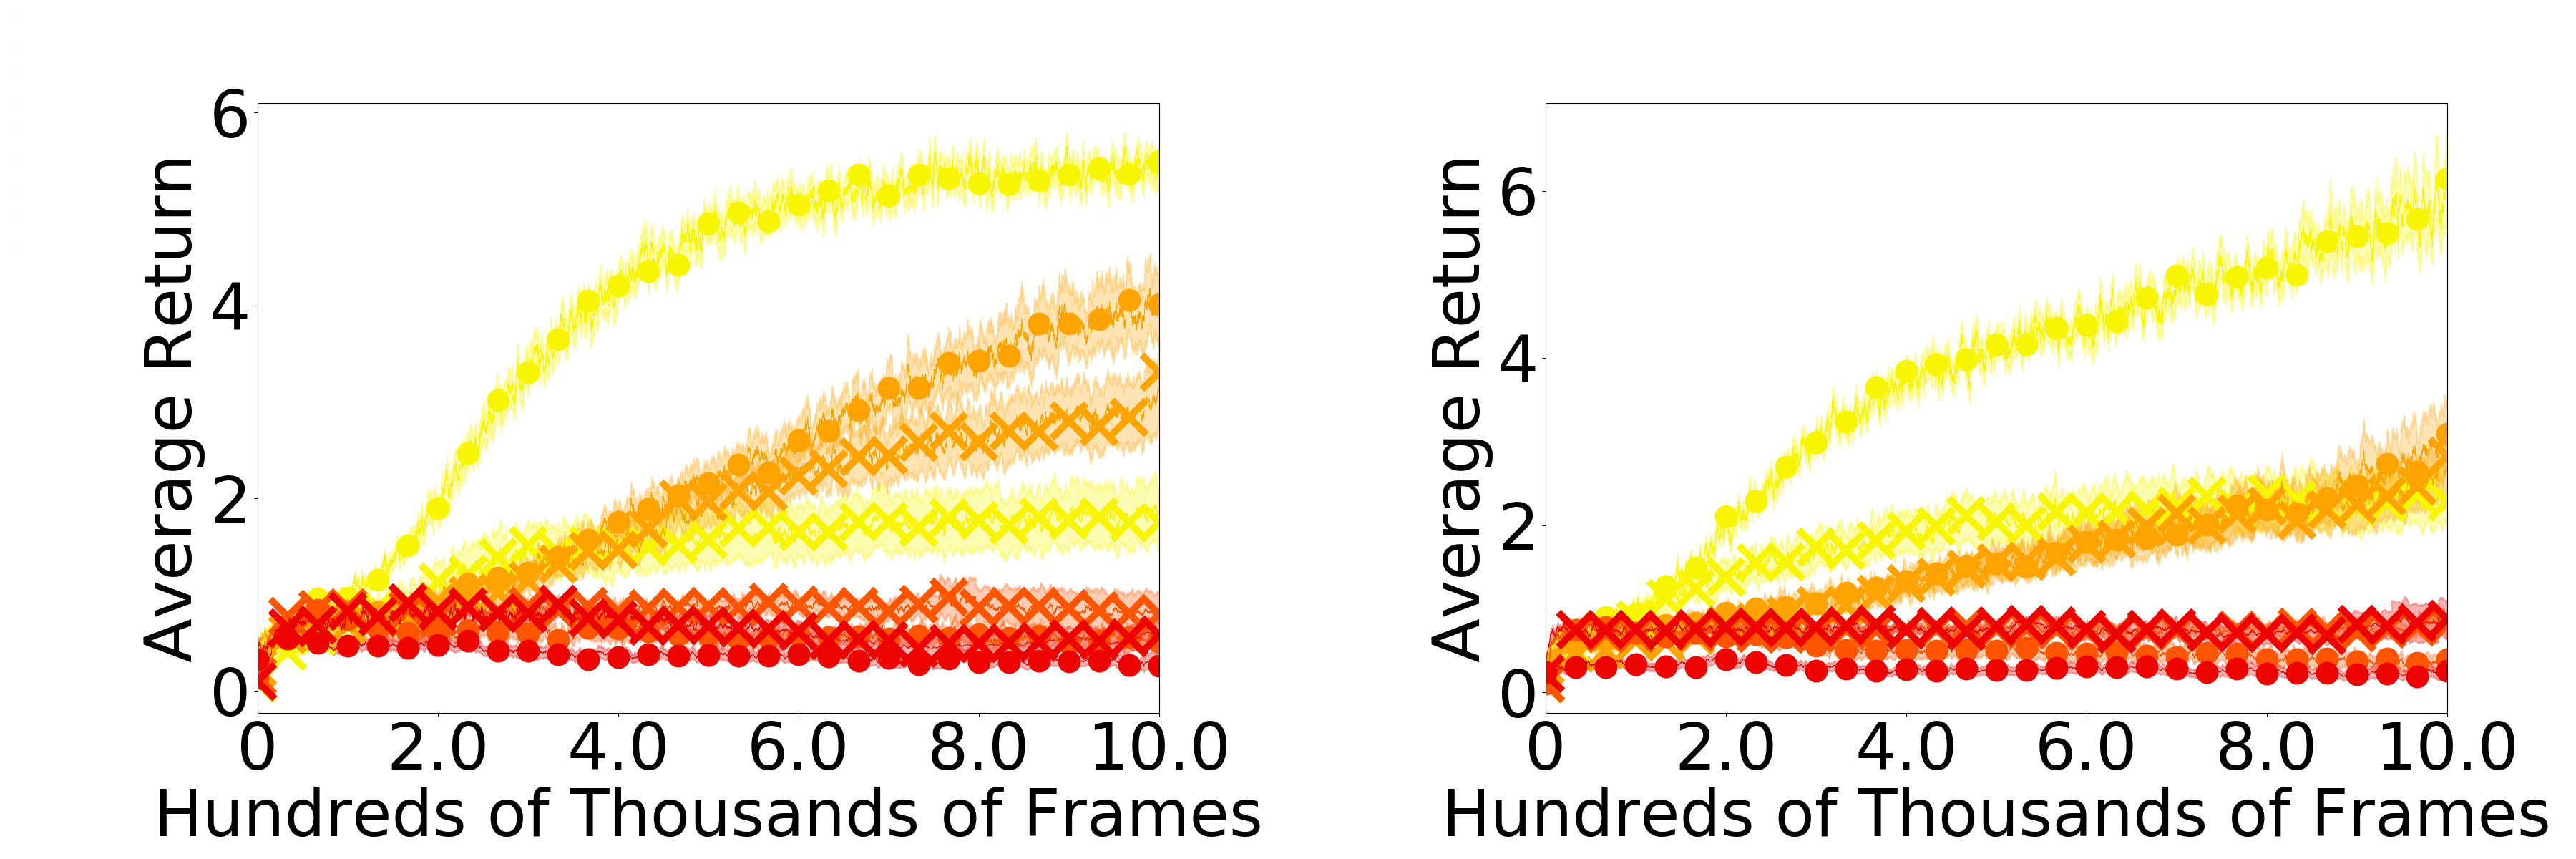
\includegraphics[width=\columnwidth]{figs/deep/discrete/seaquest_combined.png} 
    \caption{Seaquest
    }\label{fig:seaquest}
  \end{subfigure}%
  
  \begin{subfigure}[b]{1\linewidth}
    \centering
    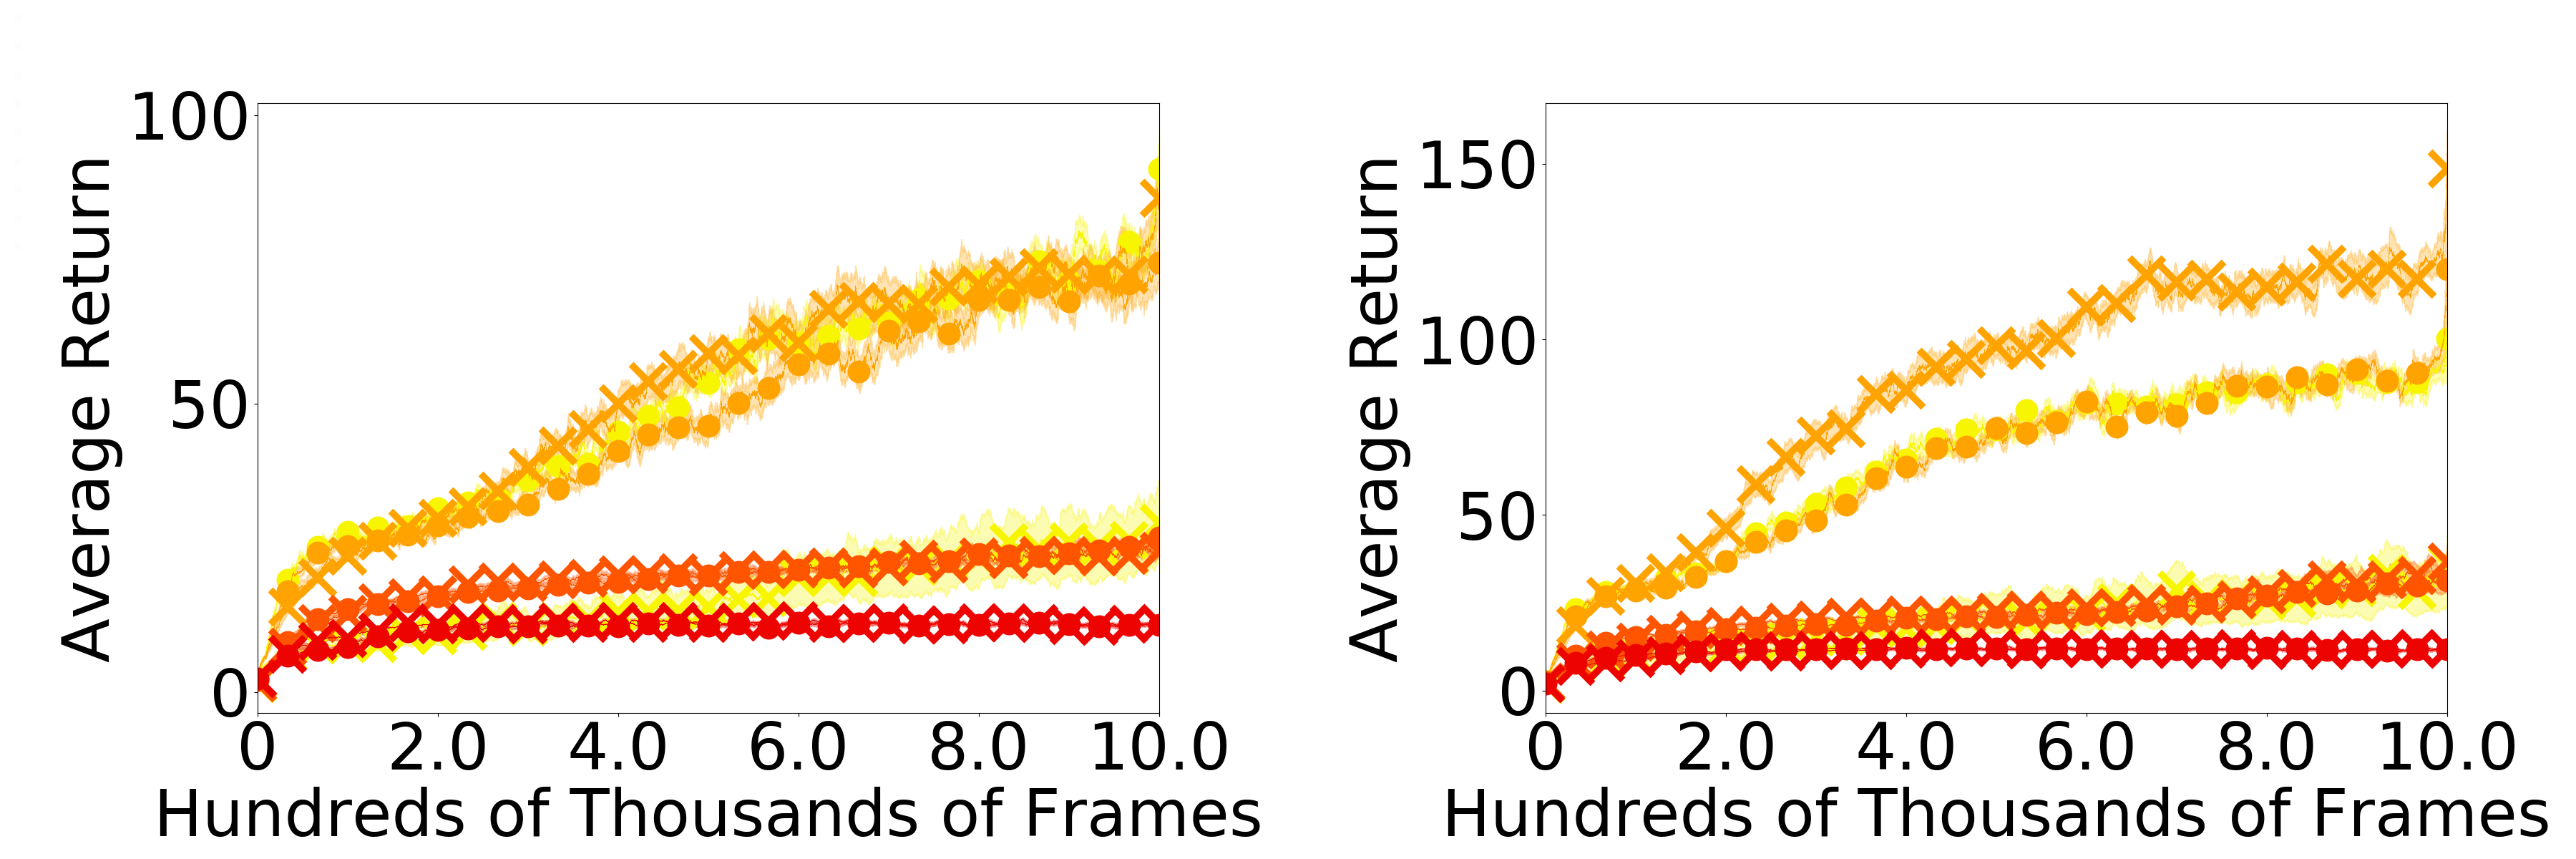
\includegraphics[width=\columnwidth]{figs/deep/discrete/space_invaders_combined.png} 
    \caption{Space Invaders
    }\label{fig:space-invaders}
  \end{subfigure}
  \caption{MinAtar discrete-action environments continued. Plot settings are identical to those in Figure \ref{fig_cont}. }\label{fig:minatar2}
\end{figure}

As with the OpenAI Gym environments, there is no consistent dominance of either KL over the other in the MinAtar environments. The most striking observation is the superiority of FKL with $\tau = 0$ over all other methods and across both hidden layer sizes on Seaquest in \Cref{fig:seaquest}. As Seaquest is generally considered to be a hard exploration problem, we might expect FKL to perform better because of its relative slowness in moving probability mass to regions with high target density, as with RKL. If this reason were the only relevant factor, we would expect FKL to be superior across all temperatures; however, FKL performs similarly to RKL for the other temperatures, excepting slightly better final performance for $\tau = 0.1$ and a hidden layer size of 32. 

Another possibility to explain the results in Seaquest is to differentiate between the supposed exploration benefits of entropy and of FKL. When we say that a method benefits exploration, we mean that the method induces a state visitation distribution whose support is larger (i.e., covers more of the state space). Accumulating more transitions from more diverse parts of the state space presumably allows for more accurate estimates of the action value function, and hence more reliable policy improvement. Entropy-regularized RL, as it is currently formulated, only benefits exploration by proxy, through penalizing the negative entropy of the policy. In the context of reward maximization, entropy is only a means to an end; at times, the means may conflict with the end. A policy with higher entropy may have a more diverse state visitation distribution, but it may be prevented from exploiting that information to the fullest capacity because of the penalty to negative entropy. In contrast, FKL benefits exploration by causing the agent's policy to commit more slowly to actions that apparently have high value under the current value function estimate. Especially since value function estimates can be atrocious \citep{ilyas2018deep}, this non-committal behaviour may help the policy avoid spurious local optima. However, FKL does not necessarily prevent a policy from committing to a particular action. Furthermore, nothing in principle prevents a policy under the hard FKL from converging to the optimal policy of the original MDP, whereas introducing entropy regularization induces a different optimal, entropy-regularized policy. 

Nevertheless, the effects of entropy and of non-committal behaviour might not be independent in all scenarios. On Freeway in \Cref{fig:freeway}, RKL bests FKL for $\tau = 0.01$, but the opposite is true for $\tau = 0$. It is conceivable that a higher temperature offsets the committal behaviour of RKL enough to impact exploration positively, while when $\tau = 0$, the RKL objective induces the policy to place large mass on actions that only appear to be optimal. A particularly striking failure case of RKL with $\tau = 0$ is on Breakout in \Cref{fig:breakout}, where this setting fails to learn appreciably compared to all other KL and $\tau$ combinations. A next step to investigate the exploration effects of entropy and of FKL would be to plot the induced state distributions of FKL and RKL over time, along with the corresponding value function estimation errors. 

\section{Summary}
We examined the differences between FKL and RKL in high-dimensional environments that necessitate function approximation. While any differences depended on the environment and the temperature, there are a few key takeaways. 
\begin{enumerate}
    \item We hypothesize that using the FKL may benefit exploration (i.e., inducing a state visitation distribution with larger support).
    \item Entropy-regularization and the FKL in conjunction may both benefit exploration, but may also inhibit learning. 
    \item The size of the hidden layer, and the function approximation architecture in general, may affect the relative superiority of FKL to RKL. 
\end{enumerate}


\end{document}